\documentclass[tikz,border=9pt]{standalone}
\usepackage{amsmath,amssymb}
\usetikzlibrary{arrows.meta,positioning,calc}
\begin{document}
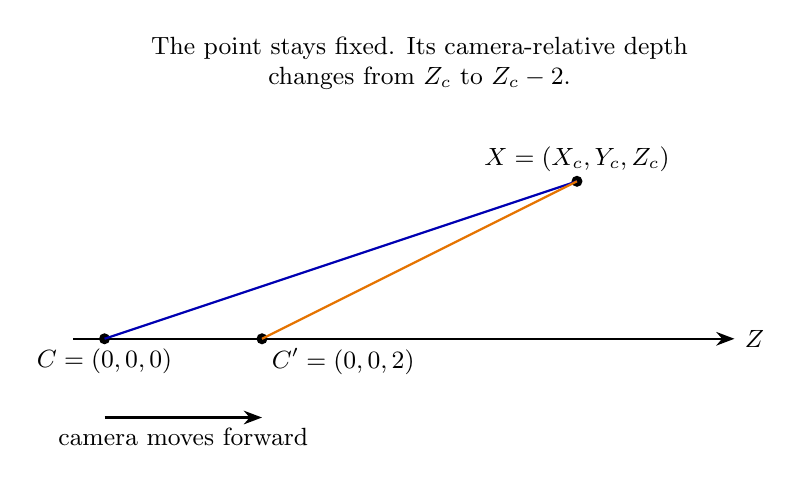
\begin{tikzpicture}[font=\small,arr/.style={-{Stealth},thick},box/.style={draw=blue!55!black,rounded corners,fill=blue!4,align=center,text width=2.9cm,minimum height=1.05cm}]

\draw[arr] (-.4,0)--(8,0) node[right]{$Z$};
\coordinate (A) at (0,0);\coordinate (B) at (2,0);\coordinate (X) at (6,2);
\fill (A) circle(2pt) node[below]{$C=(0,0,0)$};\fill (B) circle(2pt) node[below right]{$C'=(0,0,2)$};
\fill (X) circle(2pt) node[above]{$X=(X_c,Y_c,Z_c)$};
\draw[blue!70!black,thick] (A)--(X);\draw[orange!90!black,thick] (B)--(X);
\draw[arr] (0,-1)--(2,-1) node[midway,below]{camera moves forward};
\node[align=center] at (4,3.5){The point stays fixed. Its camera-relative depth\\changes from $Z_c$ to $Z_c-2$.};

\end{tikzpicture}
\end{document}
